%\documentclass[12pt][a4paper]{article}
\documentclass[twoside]{extarticle}
\usepackage{setspace}
\usepackage[latin1]{inputenc}  %verursacht komische fehler
%\usepackage[T1]{fontenc}
\usepackage[english]{babel} 
%\usepackage{blindtext}
\usepackage[top=1.5cm, bottom=2.1cm, left=2.0cm, right=2.0cm, headsep=1.4cm, includeheadfoot]{geometry}
\usepackage{fancyhdr}
\pagestyle{fancy}
\fancyhf{} % clear all



\usepackage{amsmath}
\usepackage{braket}
\usepackage[section]{placeins}
\usepackage{amsfonts}
\usepackage{amssymb}
\usepackage{graphicx}
\usepackage{parskip}
%\usepackage{subfigure}
\usepackage{subcaption}


%\usepackage{csquotes}
%\usepackage[backend=bibtex, sorting=none]{biblatex}
%\addbibresource{literature.bib}



\usepackage{pdfpages}
\usepackage{hyperref} % klicken im pdf
\usepackage{inputenc} %ermöglicht die Eingabe von Umlauten im Text, also ä, ö, ü und dem ß.
\usepackage[T1]{fontenc}
\usepackage{textcomp}
\usepackage{lmodern}
\usepackage{caption}  %damit tabellenüberschriften nicht so an den Tabellen papen
%\captionsetup[table]{skip=10pt} %damit tabellenüberschriften nicht so an den Tabellen papen
%\usepackage{units} %damit die Einheiten nicht an der Zahl pappen 
\usepackage{siunitx}


\usepackage{nomencl}
\renewcommand{\nomname}{List of Symbols}
\makenomenclature
\usepackage[titletoc, page, header]{appendix}




%\usepackage{eso-pic}
%\newcommand\BackgroundPic{
%\put(-25,0){
%\parbox[b][\paperheight]{\paperwidth}{
%\vfill
%
\includegraphics[scale=1.1]{LogoGrau.png}
%\vfill
%}}}

\begin{document}
\pagenumbering{roman} 
\begin{titlepage}
%\thispagestyle{empty}
\begin{center}
%\AddToShipoutPicture*{\BackgroundPic}
%%\doublespacing
\vspace*{2cm}
%

\begin{title}
\textbf{\textsf{\Huge Observation of Quantum Jumps in Superconducting Artificial Atoms with a Josephson Parametric Amplifier}}\\
\end{title}

\vspace*{0.5cm}

\includegraphics[width=6cm]{chapters/Introduction/figures/LogoGrau.png}
\vspace*{0.5cm}\\

%
\large {\textbf{Raffael Rabl}}\\
\large {February 2018}\\
\singlespacing
\vspace{4cm}
\large {Univ.-Prof. Dr. Gerhard Kirchmair}\\
University of Innsbruck\\
%
\vspace{1.0cm}
\large Faculty of Mathematics, Computer Science and Physics\\
\large Institute of Experimental Physics\\
\large University of Innsbruck

\end{center}
\end{titlepage}





%\newpage
%\singlespacing

%\newpage 
%%%%%%%%%%%%%%%%%%%%%
%\newpage
%\thispagestyle{empty}
%\mbox{}
%%%%%%%%%%%%%%%%%%%%%
%\newpage
%\thispagestyle{empty}
% Abstract 
%_____________________________________________________

%%\input{chapters/Abstract/abstract}

\newpage
\onehalfspace
%\thispagestyle{empty}

%_____________________________________________________
% Inhaltsverzeichnis 
%____________________________________________________

\pagestyle{empty}

\tableofcontents
\newpage

%
%\pagestyle{empty}
\printnomenclature
\newpage
\pagestyle{fancy}


\pagenumbering{arabic}
\fancyhead[RO,LE]{\nouppercase{\leftmark}} % "O" steht für "odd", also ungerade Seiten
%\fancyhead[EL]{\nouppercase{\rightmark}} % "E" für "even", also gerade Seiten.
%\fancyhead[R]{\rightmark}%
\fancyfoot[C]{\thepage}%
\renewcommand{\headrulewidth}{0.4pt}
\renewcommand{\footrulewidth}{0pt}


%_____________________________________________________
% Inhalt 
%____________________________________________________


% \input{chapters/structure/linear.tex}
% \input{chapters/structure/mixed.tex}

%\nomenclature{cavity QED}{cavity quantum electrodynamics}%
\nomenclature{QED}{quantum electrodynamics}
\nomenclature{JPC}{Josephson Parametric Amplifier}%
\nomenclature{$a$}{The number of angels per unit area}%



%-----------------------------    Chapter   -----------------------------%
\newpage

\section{Introduction}
\label{sec:introcution}



Lalalalaaa general introduction whz cQED is awesome for simulation and comp. pleeease write me! Lorem ipsum dolor sit amet, consetetur sadipscing elitr, sed diam nonumy eirmod tempor invidunt ut labore et dolore magna aliquyam erat, sed diam voluptua. At vero eos et accusam et justo duo dolores et ea rebum. Stet clita kasd gubergren, no sea takimata sanctus est Lorem ipsum dolor sit amet. Lorem ipsum dolor sit amet, consetetur sadipscing elitr, sed diam nonumy eirmod tempor invidunt ut labore et dolore magna aliquyam erat, sed diam voluptua. At vero eos et accusam et justo duo dolores et ea rebum. Stet clita kasd gubergren, no sea takimata sanctus est Lorem ipsum dolor sit amet. Lorem ipsum dolor sit amet, consetetur sadipscing elitr, sed diam nonumy eirmod tempor invidunt ut labore et dolore magna aliquyam erat, sed diam voluptua. At vero eos et accusam et justo duo dolores et ea rebum. Stet clita kasd gubergren, no sea takimata sanctus est Lorem ipsum dolor sit amet. Lorem ipsum dolor sit amet, consetetur sadipscing elitr, sed diam nonumy eirmod tempor invidunt ut labore et dolore magna aliquyam erat, sed diam voluptua. At vero eos et accusam et justo duo dolores et ea rebum. Stet clita kasd gubergren, no sea takimata sanctus est Lorem ipsum dolor sit amet. 


%To keep a clear structure I focus on the key results, and refer to the literature for derivations and in-depth analysis.


\section{Concepts}
\label{sec:concepts}

In this introductory chapter I present the key concepts, that the reader might find insightful while reading this thesis. I start with a recapitulation of cavity quantum electrodynamics (\textbf{cavity QED}) in section \ref{subsec:introduction:cavity_QED}. The central idea of this project is already developed here: determination of the quantum state of the qubit by exploiting the strong dispersive coupling between qubit and cavity. In section \ref{subsec:introduction:transmon_in_a_3D_cavity} I discuss, in what manner an artificial atom inside a 3D microwave cavity resembles such a cavity QED system. To gain an intuition about this setup, I give a brief introduction on superconducting quantum circuits. I use the simple example of a LC-oscillator, to describe, how an electronic circuit can be treated by means of quantum mechanics (section \ref{subsec:introduction:the_LC_resonator}). The most potent element of quantum circuits is the Josephson-junction (section \ref{subsec:introduction:josephson_junctions}). Its highly non-linear response, whilst being almost dissipationless, allows for the design of remarkable quantum circuits. Most notably, Josephson-junctions can be used to construct artificial atoms - quantum systems whose intrinsic parameters are controllable over a wide range during the fabrication process (section \ref{subsec:introduction:transmon}). Transition frequencies of these artificial quantum systems are typically in the microwave regime.
%TODO: spcidy f range
I introduce a few of the technical terms used in the field of microwave signal processing and describe how weak signals can be described as travelling quantum fields in section \ref{subsec:introduction:microwave_signals}. Finally I present the Josephson-parametric-converter \textbf{JPC} in section \ref{subsec:introduction:jpc}. Using this quantum-limited amplifier as first link in the amplification chain of the measurement setup significantly increases the measurement rate and allows the time-resolved observation of quantum jumps.






\subsection{Cavity QED}
\label{subsec:introduction:cavity_QED}
\cite{haroche_cavity_qed}


The theory of quantum electrodynamics (\textbf{QED}) describes the interaction between matter and light. Matter is comprised by atoms 

The quantized nature of both atoms as well as the electromagnetic field have   

The interaction between matter and light can only be understood in 




\subsubsection{Jaynes-Cummings-model}
\subsubsection{Strong dispersive regime}

\subsection{Quantum Circuits - The LC resonator}
\label{subsec:introduction:the_LC_resonator}


\subsection{Josephson junctions}
\label{subsec:introduction:josephson_junctions}

\subsection{Transmon - the artificial atom}
\label{subsec:introduction:transmon}

\subsubsection{The Cooper-pair-box CPB}
\subsubsection{Transmon regime}


\subsection{A Transmon in a 3D Cavity}
\label{subsec:introduction:transmon_in_a_3D_cavity}



\subsection{Microwave Signals}
\label{subsec:introduction:microwave_signals}

%Fortunately this frequency range lies within the operational band of telecommunication and radar systems and well developed controlling equipment is commercially available. 

\subsubsection{Classical}

\begin{itemize}
\item Transmission line 
\item SNR 
\item Amplifiers: Gain, Noise Temp, Noise figure, ...
\end{itemize}  

\subsubsection{Travelling quantum signals}

\subsection{Josephson-Parametric-Amplifier JPC}
\label{subsec:introduction:jpc}

\subsubsection{Josephson ring modulator}
\subsubsection{Scattering matrix}





%-----------------------------    Chapter   -----------------------------%
%\newpage
%\section{Circuit QED}
%\label{sec:circuit_qed}
%
%\subsection{Concepts}
%\label{subsec:circuit_qed:concepts}
%\input{chapters/Circuit_QED/Concepts.tex}
%
%\subsection{Microwave Cavities as Quantum Systems}
%\label{subsec:circuit_qed:microwave_cavities}
%\input{chapters/Circuit_QED/Microwave_Cavities.tex}
%
%\subsection{The Transmon}
%\label{subsec:circuit_qed:the_transmon}
%\input{chapters/Circuit_QED/The_Transmon.tex}
%
%\subsection{Coupled System - A Transmon in a Cavity}
%\label{subsec:circuit_qed:transmon_in_a_cavity}
%\input{chapters/Circuit_QED/Coupled_System.tex}
%


%-----------------------------    Chapter   -----------------------------%
%\newpage
%\section{Cavity QED}
%\label{sec:cavity_QED}
%
%\subsection{Jaynes-Cummings-Model}
%\label{subsec:cavity_QED:jaynes-cummings-model}
%\input{chapters/Cavity_QED/Jaynes-Cummings-Model.tex}
%
%\subsection{Dispersive Regime}
%\label{subsec:cavity_QED:dispersive_regime}
%\begin{figure}[htb]
    \centering
        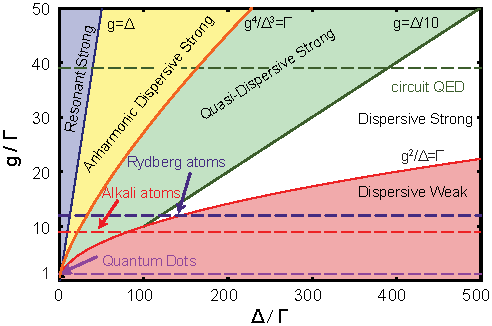
\includegraphics[width=8.6cm]{chapters/Cavity_QED/figures/regimes_of_cavity_QED.pdf}
        \caption{Regimes od Cavity QED \cite{phd_thesis_schuster}.}
        \label{fig:schaukel}
\end{figure}





%






%-----------------------------    Chapter   -----------------------------%
\newpage
\section{Characterising the System}
\label{sec:characterizing_the_system}

\subsection{Experimental Setup}
\label{sec:characterizing_the_system:experimental_setup}
\input{chapters/Characterizing_the_System/Experimental_Setup.tex}

\FloatBarrier
\subsection{Cavity Spectroscopy}
\label{sec:characterizing_the_system:cavity_spectroscopy}



\subsubsection{From High Power to Low Power}
\label{subsec:characterizing_the_system:from_high_to_low_power}



\begin{figure}[htb!]
\centering
\includegraphics[width=17.2cm]{plots/qubit_spectroscopy/spectra/low_and_high_power.pdf}
\caption{
Reflection spectrum of the cavity taken with a VNA for high (blue) and low power (orange). In the low-power-measurement the average excitation of the cavity filed amounts to roughly $10$ (check this number!) photons. The observed lamb-shift of the resonance frequency is due to the coupling between cavity and transmon.
}
\label{fig:cavity_spectroscopy:from_high_to_power}
\end{figure}







\subsubsection{Driving the Transmon}



\begin{figure}
\centering
\includegraphics[width=17.2cm]{plots/qubit_spectroscopy/multi_plots/fluxmap_qubit_ge_AND_qubit_peak.png}
\caption{testcaption}
\label{testlabel}
\end{figure}




%\begin{figure}
%\centering
%\subcaptionbox{
%Averaged VNA reflection measurements of the cavity (y-axis) while driving the qubit at different frequencies (x-axis).
%\label{fig:cavity_spectroscopy:qubit_ge:contour}}
%[8.6cm]{\includegraphics[width=8.6cm]{plots/qubit_spectroscopy/fluxmaps/driving_ge.pdf}}
%~
%\subcaptionbox{
%Horizontal cut at $f_\text{c}-\chi$ (dashed line). A lorentzian fit of the linearized data yields the qubit frequency $f_\text{01} = \SI{6.449}{GHz}$. 
%\label{fig:cavity_spectroscopy:qubit_ge:horizontal}}
%[8.6cm]{\includegraphics[width=8.6cm]{plots/qubit_spectroscopy/spectra/qubit_ge_transition.pdf}}
%~
%\subcaptionbox{
%A vertical cut at $f_\text{01}$ shows the appearance of the cavity peak corresponding to the excited state of the transmon in the averaged VNA spectrum.
%\label{fig:cavity_spectroscopy:qubit_ge:vertical}}
%[8.6cm]{\includegraphics[width=8.6cm]{plots/qubit_spectroscopy/spectra/two_peaks_low_power.pdf}}
%~
%\subcaptionbox{
%Another VNA spectrum with a stronger qubit driven almost in saturation, as seen by the equal heights of the dips. The dispersive shift is determined by fitting a lorentzian profile two each resonance.
%\label{fig:cavity_spectroscopy:qubit_ge:vertical_more_drive_power}}
%[8.6cm]{\includegraphics[width=8.6cm]{plots/qubit_spectroscopy/spectra/two_peaks_high_power.pdf}}
%\caption{
%Reflection spectrum of the cavity with an additional drive tone to probe the qubit. The qubit drive frequency is iterated in steps of $\SI{100}{kHz}$ from $\SI{6.44}{GHz}$ to $\SI{6.46}{GHz}$ . For each frequency a low power VNA-spectrum with $100$ averages is performed. The reflected magnitude is shown in the contour plot (\subref{fig:cavity_spectroscopy:qubit_ge:contour}). A horizontal cut at $f_\text{c}-\chi$ (dashed line) reveals the qubit resonance at $f_\text{01} = \SI{6.449}{GHz}$ (\subref{fig:cavity_spectroscopy:qubit_ge:horizontal}). Driving the qubit at this frequency populates the first excited level of the transmon. Therefore the cavity resonance corresponding to the excited transmon state becomes more prominent (\subref{fig:cavity_spectroscopy:qubit_ge:vertical}), and even more so for a stronger qubit drive power (\subref{fig:cavity_spectroscopy:qubit_ge:vertical_more_drive_power}).
%}
%\label{fig:cavity_spectroscopy:qubit_ge:main}
%\end{figure}





\begin{figure}
\centering
\includegraphics[width=17.2cm]{plots/qubit_spectroscopy/multi_plots/two_cavity_peaks_different_drives.pdf}
\caption{testcaption}
\label{testlabel}
\end{figure}





\begin{figure}
\centering
\includegraphics[width=17.2cm]{plots/qubit_spectroscopy/multi_plots/fluxmap_qubit_ef_AND_cavity_3_peak_spectrum.png}
\caption{testcaption}
\label{testlabel}
\end{figure}





%
%
%
%\begin{figure}
%\centering
%\subcaptionbox{
%Averaged VNA reflection measurements of the cavity (y-axis) while driving the ge-transition on resonance to populate the excited state of the transmon. Applying an additional RF probe reveals the ef-transition at roughly $\SI{6.177}{GHz}$ (vertical dashed line)
%\label{fig:cavity_spectroscopy:qubit_ef:contour}}
%[8.6cm]{\includegraphics[width=8.6cm]{plots/qubit_spectroscopy/fluxmaps/driving_ef.pdf}}
%~
%\subcaptionbox{
%vertical cut through (\subref{fig:cavity_spectroscopy:qubit_ef:contour}) at $f_\text{c}-\chi$ (dashed line). Driving the ge- and the ef-transition at the same time populates both the $\ket{e}$ and the $\ket{f}$ state of the transmon. The respective peaks appear in the averaged cavity spectrum.
%\label{fig:cavity_spectroscopy:qubit_ef:vertical}}
%[8.6cm]{\includegraphics[width=8.6cm]{plots/qubit_spectroscopy/spectra/three_peaks.pdf}}
%\caption{
%VNA reflection measurement of the cavity with two additional RF tones applied to find the ef-transition of the transmon. Each VNA trace consists of $100$ averages.
%}
%\label{fig:cavity_spectroscopy:qubit_ef:main}
%\end{figure}
%


\begin{figure}
\centering
{\includegraphics[width=8.6cm]{plots/qubit_spectroscopy/spectra/three_peaks_lin.pdf}}
\caption{
Same as above but linear $P_{in}/P_{out}$ data.
}
\label{fig:cavity_spectroscopy:qubit_ef:main}
\end{figure}




\FloatBarrier


\subsection{Summary of System Parameters}
\label{sec:characterizing_the_system:summary_of_experimental_params}

\begin{table}[htb!]
\centering
\begin{tabular}{c|c|c} 
Description   &   Symbol       & Value                                     \\ 
\hline
Cavity when transmon in $\ket{g} $   &   $\omega _\text{c} ^{\text{g}} / 2 \pi $      &    $\SI{8.809641 (2) }{GHz}$                   \\ 
\hline
Cavity when transmon in $\ket{e} $   &   $\omega _\text{c} ^{\text{e}} / 2 \pi $      &    $\SI{8.806588 (3) }{GHz}$                   \\ 
\hline
Cavity when transmon in $\ket{f} $   &   $\omega _\text{c} ^{\text{f}} / 2 \pi $      &    $\SI{8.803983 (3) }{GHz}$                   \\ 
\hline
Dispersive shift                     &   $\chi /2 \pi $                                 &    $\SI{3.053 (5) }{MHz}$                    \\ 
\hline
Cavity decay rate                     &   $\kappa /2 \pi $                                 &    $\SI{2.096 (5) }{MHz}$                 \\ 
\hline
Transmon $\ket{g} \leftrightarrow  \ket{e}$ transition   &   $\omega _\text{ge}  / 2 \pi $      &    $\SI{6.4500 (3) }{GHz}$           \\ 
\hline
Transmon $\ket{e} \leftrightarrow \ket{f}$ transition   &   $\omega _\text{ef}  / 2 \pi $      &    $\SI{6.177 (2) }{GHz}$             \\ 
\hline
Anharmonicity                         &   $\alpha  / 2 \pi $                                 &         $\SI{273}{MHz}$                 \\ 
\hline
Qubit dephasing                       & $\Gamma$                                          &                                            \\
\end{tabular} 
\caption{ Experimentally determined parameters of the transmon-cavity-system.  }
\label{tab:variablen}
\end{table}







%-----------------------------    Chapter   -----------------------------%
\newpage
\section{Cranking up the Contrast: The Josephson Parametric Amplifier}

\subsection{Travelling Quantum Signals}

\subsection{Operational Principle}

\subsubsection{The Josephson Ring Modulator}

\subsubsection{A Chain of Amplifiers}

\subsection{Tuning Procedure}
\label{sec:jpc:tuning_procedure}
\subsubsection{Fluxmaps}




\begin{figure}
    \centering
    \begin{subfigure}[b]{8.6cm}
        \includegraphics[width=\textwidth]{plots/jpc/fluxmaps/quantumcircuits_signal.pdf}
        \caption{A gull}
        \label{fig:jpc:fluxmaps:reference:signal_resonator}
    \end{subfigure}
    ~ %add desired spacing between images, e. g. ~, \quad, \qquad, \hfill etc. 
      %(or a blank line to force the subfigure onto a new line)
    \begin{subfigure}[b]{8.6cm}
        \includegraphics[width=\textwidth]{plots/jpc/fluxmaps/quantumcircuits_idler.pdf}
        \caption{A tiger}
        \label{fig:jpc:fluxmaps:reference:idler_resonator}
    \end{subfigure}
    \caption{Pictures of animals}\label{fig:jpc:fluxmaps:reference:main}
\end{figure}



\begin{figure}[htb!]
    \centering
        \includegraphics[width=8.6cm]{plots/jpc/fluxmaps/measured_fluxmap_full_range.pdf}
        \caption{Measured Fluxmap of the JPC SN004.}
        \label{fig:jpc:fluxmaps:measured_signal_resonator}
\end{figure}






\FloatBarrier
\subsubsection{Controlling the Gain}




\begin{figure}
\centering
\subcaptionbox{
Phase response of the signal reflected by the JPC signal resonator for three different bias currents while the pump is off.
\label{fig:jpc:tuning:signal_phase_response}}
[8.6cm]{\includegraphics[width=8.6cm]{plots/jpc/tuning/signal_resonator_phase_response.pdf}}
~
\subcaptionbox{
Magnitude of the reflected signal for the same bias current as in (\subref{fig:jpc:tuning:signal_phase_response}) with pump tuned accordingly, to produce a gain. The dips in the data are due to qubits in the waveguide.
\label{fig:jpc:tuning:gain_over_the_whole_range}}
[8.6cm]{\includegraphics[width=8.6cm]{plots/jpc/tuning/gain_curve_sweep.pdf}}
\caption{Controlling the position of the central JPC gain frequency. The signal-resonator is tuned via the bias current until it covers the desired frequency (a). Then the JPC-pump is turned on and its power is carefully increased (a). The gain should be visible in transmission if the frequency matching condition $\omega_\text{S} + \omega_\text{I} = \omega_\text{P}$ is fulfilled. If no gain appears, the pump has to be set to a slightly different frequency with its power again slowly swept from low to high. A decent guess for $\omega_\text{P}$ can be obtained from the provided reference fluxmaps \ref{fig:jpc:fluxmaps:reference:main} for the signal and idler resonator of the JPC.}
\label{fig:jpc:tuning:main}
\end{figure}



\begin{figure}
\centering
{\includegraphics[width=8.6cm]{plots/jpc/tuning/gain_sweep.pdf}}
\caption{Gain curve of the JPC for different pump powers.
}
\label{fig:jpc:tuning:low_gain_to_high_gain}
\end{figure}







\FloatBarrier
\subsection{Testing the JPC SN004}
\label{sec:jpc:testing_the_SN004}
\subsubsection{Noise Rise}
\FloatBarrier


\begin{figure}
\centering
\subcaptionbox{
Calibrated reflection measurement of the JPC. Fitting a lorentzian reveals a gain of $\SI{13}{dB}$ at $\SI{8.974}{GHz}$.
\label{fig:jpc:noise_rise:jpc_gain}}
[8.6cm]{\includegraphics[width=8.6cm]{{plots/jpc/noise_rise/vna_spectrum_9.9GHz_20.0dB_gain}.pdf}}
~
\subcaptionbox{
Spectral power density coming out of the signal port of the JPC, measured with a spectrum analyser (subtracted background). The JPC is operated with the same parameters as in (\subref{fig:jpc:noise_rise:jpc_gain}). The noise added by the JPC is clearly visible.
\label{fig:jpc:noise_rise:spectrum_analyser}}
[8.6cm]{\includegraphics[width=8.6cm]{{plots/jpc/noise_rise/noise_spectrum_9.9GHz_20.0dB_gain}.pdf}}
\caption{JPC gain: 20dB, NVR: 13.1dB ... Please measure me again!}
\label{fig:jpc:noise_rise:main}
\end{figure}









\FloatBarrier




%-----------------------------    Chapter   -----------------------------%
\newpage
\section{Observing Quantum Jumps}

\subsection{Heterodyne Detection Setup}
\label{sec:quantum_jumps:heterodyne_detection_setup}
\subsubsection{Digital Demodulation Scheme}



\begin{figure}
\centering
\subcaptionbox{
caption 111
\label{fig:IQ:first_measurements:asdfasdf}}
[8.6cm]{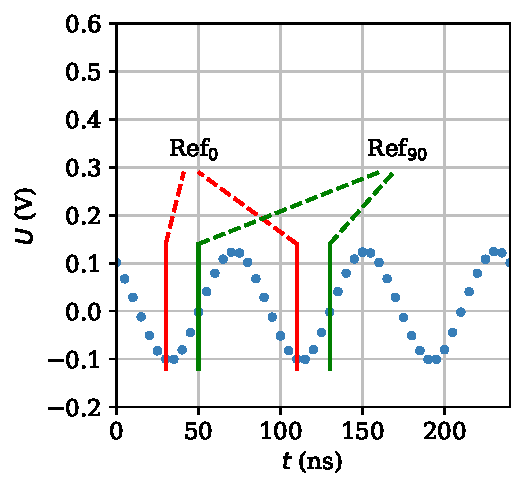
\includegraphics[width=8.6cm]{plots/IQ_plots/demodulation_sheme/ref_wave.pdf}}
~
\subcaptionbox{
caption 111
\label{fig:IQ:first_measurements:asdfasdf}}
[8.6cm]{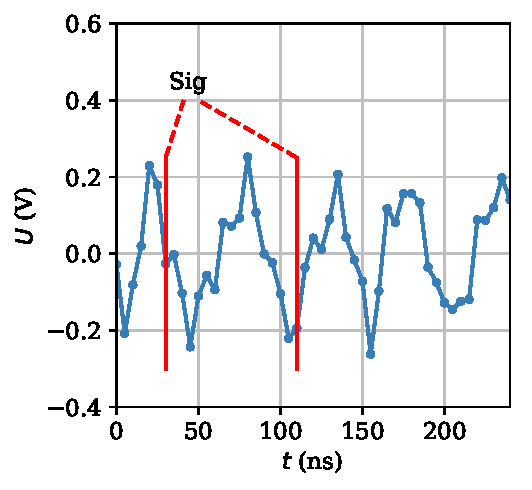
\includegraphics[width=8.6cm]{plots/IQ_plots/demodulation_sheme/sig_wave.pdf}}
\caption{main caption}
\label{fig:jpc:noise_rise:main}
\end{figure}

\FloatBarrier



\subsection{Resolving Quantum States in the IQ-Plane}
\label{sec:quantum_jumps:resolving_quantum_states_in_the_iq_plane}
\subsubsection{First Measurements}





\begin{figure}
\centering
\subcaptionbox{
Scatter plot of $10000$ IQ-records with an alpha value of $0.1$ while the JPC is turned off.
\label{fig:IQ:first_measurements:IQ_jpc_off}}
[8.6cm]{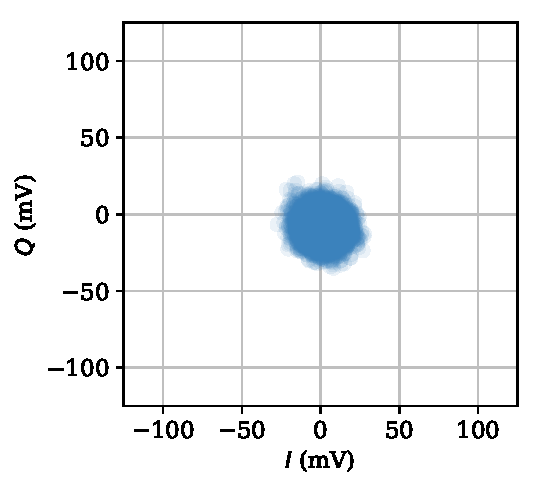
\includegraphics[width=8.6cm]{plots/IQ_plots/first_measurements/IQ_jpc_off.pdf}}
~
\subcaptionbox{
Transmission spectra of the cavity measured with a VNA while the JPC is turned off (orange) and on (blue). The JPC is operated with a gain of $\SI{27}{dB}$ at the IQ-readout frequency (dashed black line).
\label{fig:IQ:first_measurements:JPC_curves}}
[8.6cm]{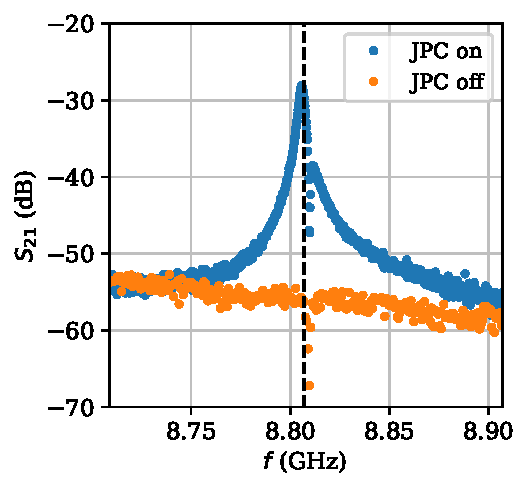
\includegraphics[width=8.6cm]{plots/IQ_plots/first_measurements/vna_jpc_on_off.pdf}}
~
\subcaptionbox{
Same measurement as in (\subref{fig:IQ:first_measurements:IQ_jpc_off}) with JPC turned on. The improvement in SNR clearly resolved three distinct features.
\label{fig:IQ:first_measurements:IQ_jpc_on}}
[8.6cm]{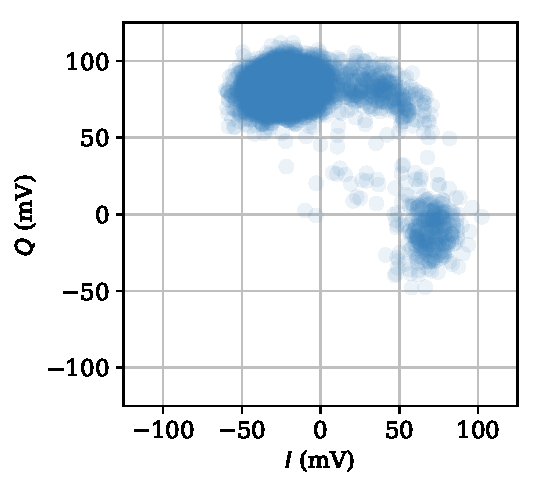
\includegraphics[width=8.6cm]{plots/IQ_plots/first_measurements/IQ_jpc_on.pdf}}
\caption{
First IQ-measurements with $T_{mes} = \SI{640}{ns}$ at $P_{mes} = \SI{16}{dBm}$ and a probe frequency $f_{P} = \SI{8.8069}{GHz}$. Without the JPC the cahracteristic features, that would indicate the quantum state of the system, remain hidden in the noise (\subref{fig:IQ:first_measurements:IQ_jpc_off}). Turning on the JPC with the maximum gain frequency tuned to the IQ readout frequency $f_{P}$ (\subref{fig:IQ:first_measurements:JPC_curves}) increases the SNR and reveals three distinct spots at which the individual measurement records accumulate (\subref{fig:IQ:first_measurements:IQ_jpc_on}). Their distribution clearly deviate from the expected gaussian shape. This is due to the high readout-power and hard driving of the JPC.}
\label{fig:IQ:first_measurements:main}
\end{figure}

\FloatBarrier


\subsection{Improving the Contrast}
\label{sec:quantum_jumps:improving_the_contrast}
\FloatBarrier
\subsubsection{Analysing IQ-data: Figures of merit}




\begin{figure}
\centering
{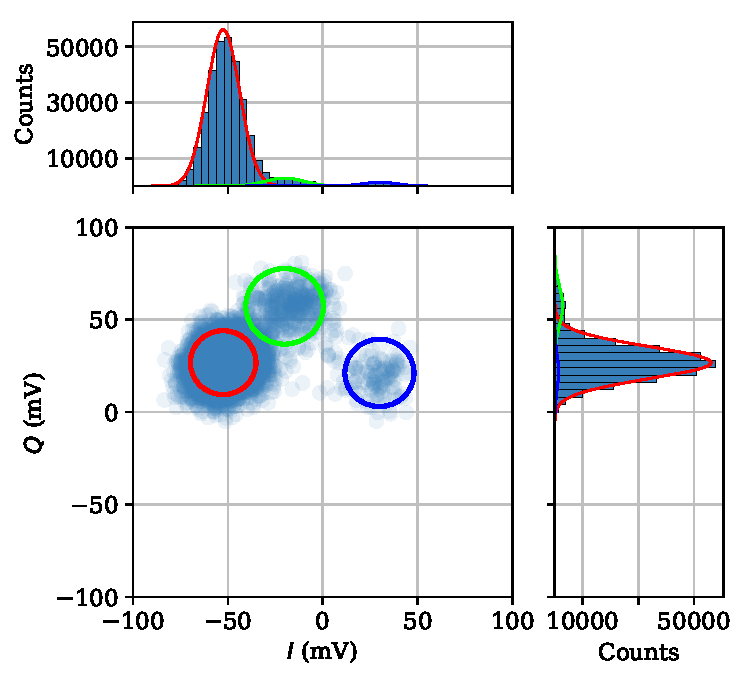
\includegraphics[width=12.9cm]{plots/IQ_plots/figures_of_merit/awesome_multiplot.pdf}}
\caption{
IQ-measurement with $T_{mes} = \SI{640}{ns}$ at $P_{mes} = \SI{24}{dBm}$ and $330000$ points. The scatter plot shows the first $10000$ data points with an alpha value of $0.1$. The circles represent the $2\sigma$-radius of the gaussian profiles obtained by fitting the 2D-histogram as described above. The histograms are computed by binning the $I$- respectively the $Q$-component of each individual measurement record of the full data set into $50$ intervals of equal length. The coloured lines again show the gaussian profiles of the corresponding disk, as achieved from fitting the 2D-model, but the amplitude is corrected by a scaling factor of $\sqrt{2 \pi \sigma^2}$ times the bin-width to account for the projection onto the respective axis.
}
\label{fig:IQ:figures_of_merit:awesome_multiplot}
\end{figure}









\begin{figure}
\centering
\subcaptionbox{
Scatter plot of the IQ-data with $2\sigma\text{-radius}$ of the fitted gaussian profiles.
\label{fig:IQ:figures_of_merit:scatter}}
[8.6cm]{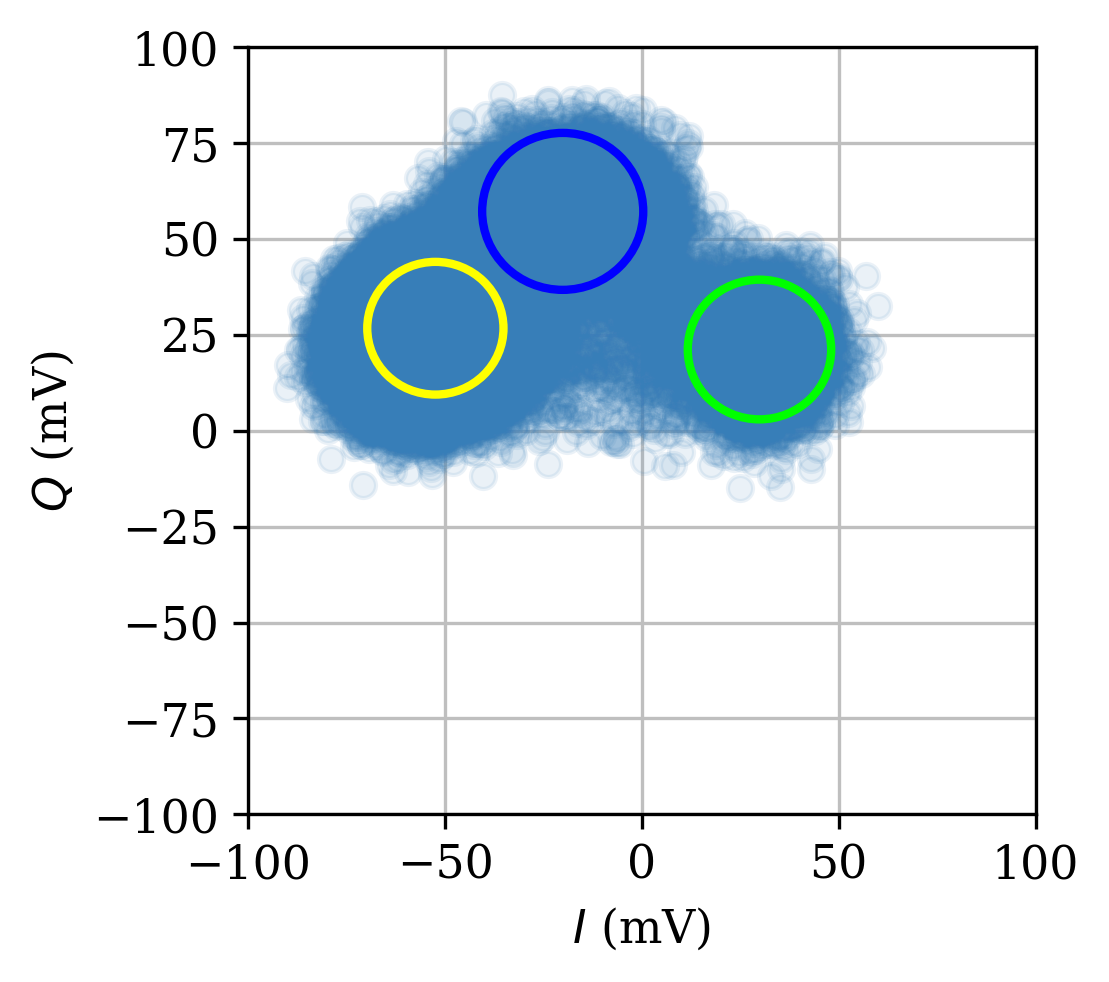
\includegraphics[width=8.6cm]{plots/IQ_plots/figures_of_merit/scatter_plot.pdf}}
~
\subcaptionbox{
Logarithmic histogram of the binned IQ-data.
\label{fig:IQ:figures_of_merit:2D_histo}}
[8.6cm]{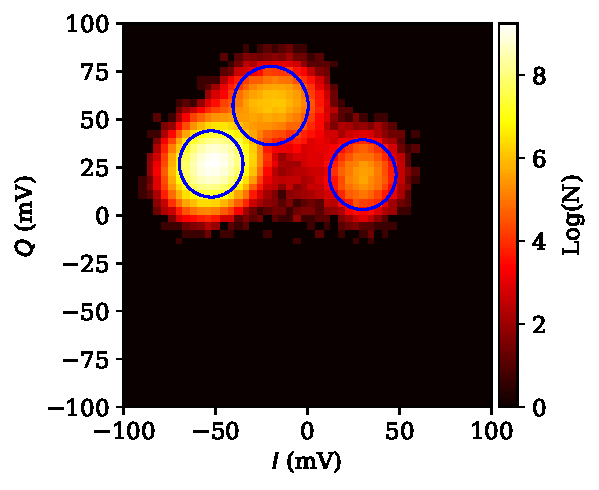
\includegraphics[width=8.6cm]{plots/IQ_plots/figures_of_merit/histo_log.pdf}}
~
\subcaptionbox{
Cumulative projection of the binned data onto the $Q$- and $I$-axis and the gaussian envelopes of the respective disks. The colors are the same as in (\subref{fig:IQ:figures_of_merit:scatter}), the sum of the three gaussians is shown in red.
\label{fig:IQ:figures_of_merit:projected_histo_lin}}
[8.6cm]{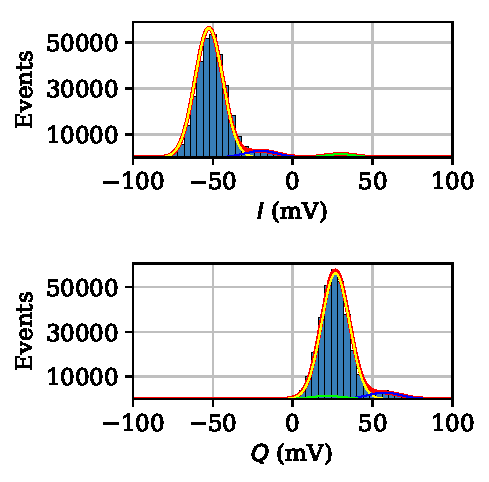
\includegraphics[width=8.6cm]{plots/IQ_plots/figures_of_merit/projected_histo_lin_combined_plot.pdf}}
~
\subcaptionbox{
Projection of the logarithmic histogram. Does this even make sense?
\label{fig:IQ:figures_of_merit:projected_histo_log}}
[8.6cm]{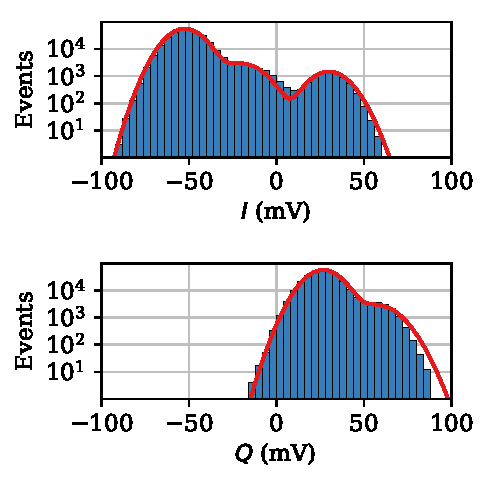
\includegraphics[width=8.6cm]{plots/IQ_plots/figures_of_merit/projected_histo_log_combined_plot.pdf}}
\caption{
IQ-measurement with $T_{mes} = \SI{640}{ns}$ at $P_{mes} = \SI{24}{dBm}$ and $330000$ points. In order to quantify the separation and the spread of the disks, that represent the different quantum states, I bin the results onto a 2D-histogram and perform a least-square-fit with the sum of three gaussian profiles.
}
\label{fig:IQ:figures_of_merit:main}
\end{figure}







\FloatBarrier
\subsubsection{Readout Power Sweep}

%
%
%\begin{figure}
%\centering
%\subcaptionbox{
%caption 111
%\label{fig:IQ:improving_contrast:readout_power:1}}
%[4.0cm]{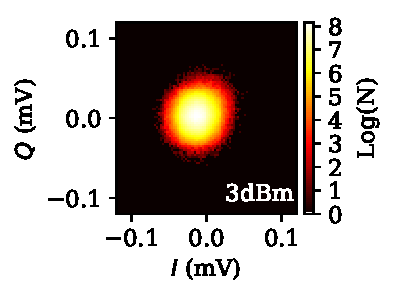
\includegraphics[width=4.0cm]{plots/IQ_plots/contrast_sweeps/readout_power/3dBm.pdf}}
%~
%\subcaptionbox{
%caption 111
%\label{fig:IQ:improving_contrast:readout_power:2}}
%[4.0cm]{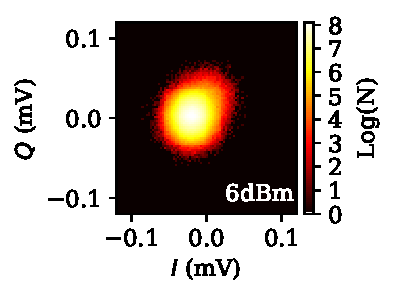
\includegraphics[width=4.0cm]{plots/IQ_plots/contrast_sweeps/readout_power/6dBm.pdf}}
%~
%\subcaptionbox{
%caption 111
%\label{fig:IQ:improving_contrast:readout_power:2}}
%[4.0cm]{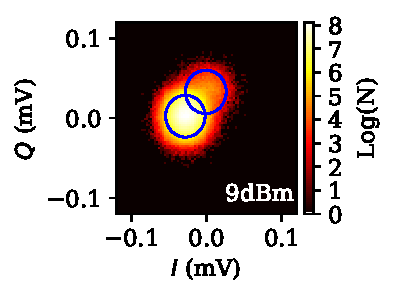
\includegraphics[width=4.0cm]{plots/IQ_plots/contrast_sweeps/readout_power/9dBm.pdf}}
%~
%\subcaptionbox{
%caption 111
%\label{fig:IQ:improving_contrast:readout_power:2}}
%[4.0cm]{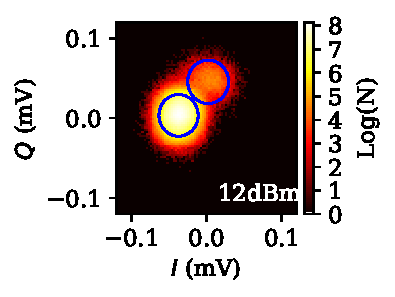
\includegraphics[width=4.0cm]{plots/IQ_plots/contrast_sweeps/readout_power/12dBm.pdf}}
%~
%\subcaptionbox{
%caption 111
%\label{fig:IQ:improving_contrast:readout_power:2}}
%[4.0cm]{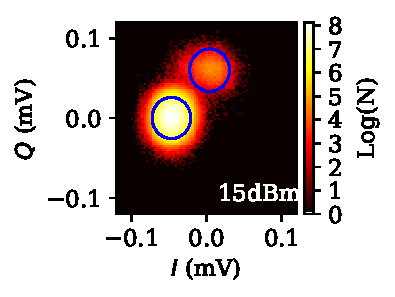
\includegraphics[width=4.0cm]{plots/IQ_plots/contrast_sweeps/readout_power/15dBm.pdf}}
%~
%\subcaptionbox{
%caption 111
%\label{fig:IQ:improving_contrast:readout_power:2}}
%[4.0cm]{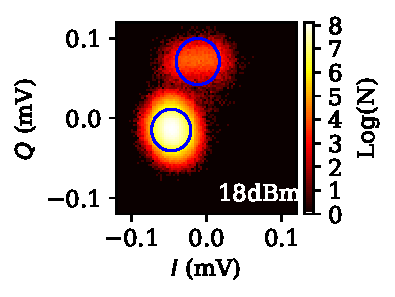
\includegraphics[width=4.0cm]{plots/IQ_plots/contrast_sweeps/readout_power/18dBm.pdf}}
%~
%\subcaptionbox{
%caption 111
%\label{fig:IQ:improving_contrast:readout_power:2}}
%[4.0cm]{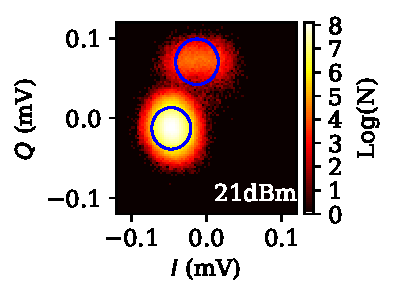
\includegraphics[width=4.0cm]{plots/IQ_plots/contrast_sweeps/readout_power/21dBm.pdf}}
%~
%\subcaptionbox{
%caption 111
%\label{fig:IQ:improving_contrast:readout_power:2}}
%[4.0cm]{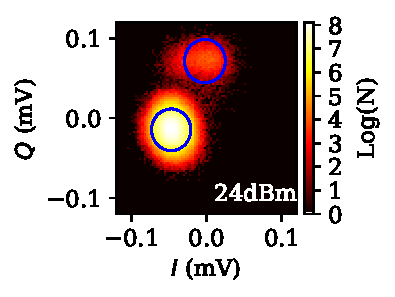
\includegraphics[width=4.0cm]{plots/IQ_plots/contrast_sweeps/readout_power/24dBm.pdf}}
%\caption{main caption}
%\label{fig:jpc:noise_rise:main}
%\end{figure}
%

\FloatBarrier
\subsubsection{Readout Time}

%
%\begin{figure}
%\centering
%\subcaptionbox{
%caption 111
%\label{fig:IQ:improving_contrast:readout_time:1}}
%[4.0cm]{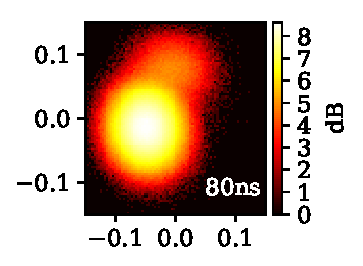
\includegraphics[width=4.0cm]{plots/IQ_plots/contrast_sweeps/readout_time/80ns.pdf}}
%~
%\subcaptionbox{
%caption 111
%\label{fig:IQ:improving_contrast:readout_time:1}}
%[4.0cm]{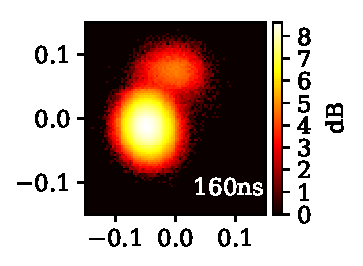
\includegraphics[width=4.0cm]{plots/IQ_plots/contrast_sweeps/readout_time/160ns.pdf}}
%~
%\subcaptionbox{
%caption 111
%\label{fig:IQ:improving_contrast:readout_time:1}}
%[4.0cm]{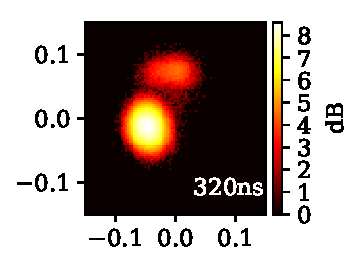
\includegraphics[width=4.0cm]{plots/IQ_plots/contrast_sweeps/readout_time/320ns.pdf}}
%~
%\subcaptionbox{
%caption 111
%\label{fig:IQ:improving_contrast:readout_time:1}}
%[4.0cm]{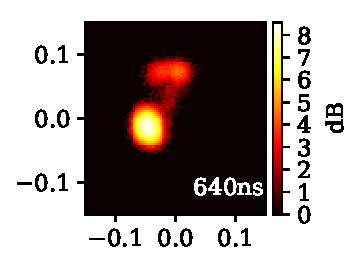
\includegraphics[width=4.0cm]{plots/IQ_plots/contrast_sweeps/readout_time/640ns.pdf}}
%\caption{main caption}
%\label{fig:jpc:noise_rise:main}
%\end{figure}

\FloatBarrier

\subsection{Monitoring the State in Time}
\label{sec:quantum_jumps:monitoring_the_state_in_time}
\FloatBarrier

\begin{figure}
\centering
\subcaptionbox{
$T_{\text{mes}} = \SI{160}{ns}$.
\label{fig:quamtum_jumps:IQ_160ns}}
[8.6cm]{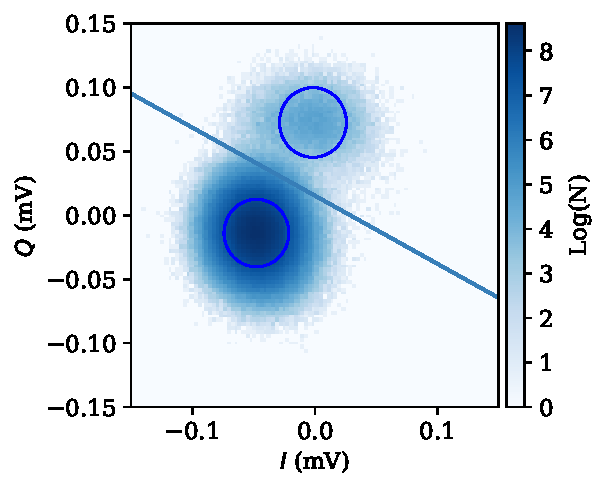
\includegraphics[width=8.6cm]{plots/IQ_plots/quantum_jumps/2_discs_super_nice.pdf}}
~
\subcaptionbox{
$T_{\text{mes}} = \SI{160}{ns}$.
\label{fig:quamtum_jumps:jumptrace_160ns}}
[8.6cm]{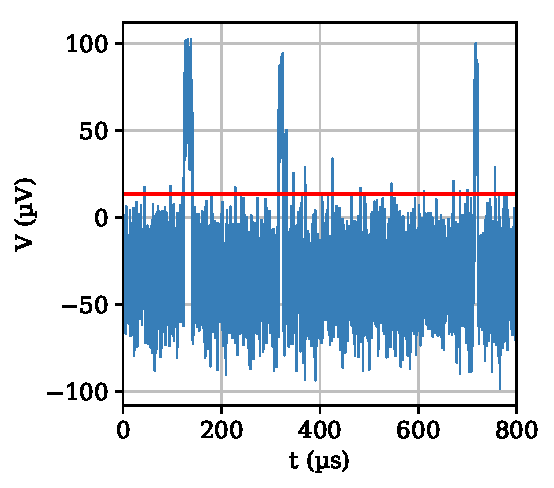
\includegraphics[width=8.6cm]{plots/IQ_plots/quantum_jumps/long_trace_1_avg.pdf}}
~
\subcaptionbox{
$T_{\text{mes}} = \SI{320}{ns}$.
\label{fig:quamtum_jumps:IQ_320ns}}
[8.6cm]{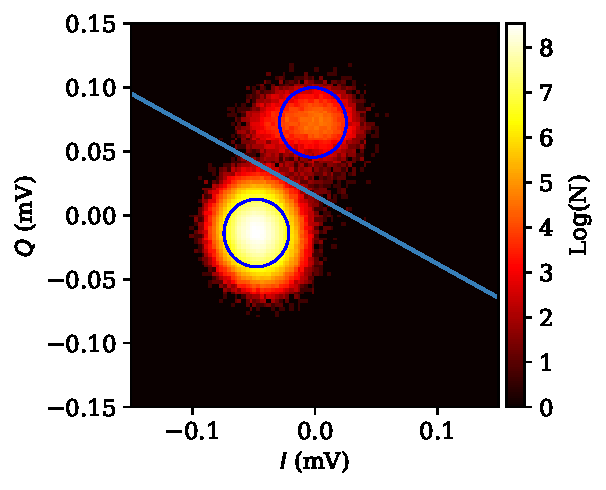
\includegraphics[width=8.6cm]{plots/IQ_plots/quantum_jumps/2_discs_super_nice_2_avg.pdf}}
~
\subcaptionbox{
$T_{\text{mes}} = \SI{320}{ns}$.
\label{fig:quamtum_jumps:jumptrace_320ns}}
[8.6cm]{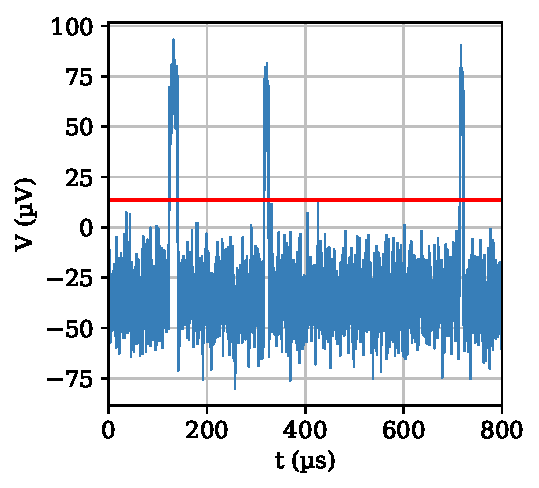
\includegraphics[width=8.6cm]{plots/IQ_plots/quantum_jumps/long_trace_2_avg.pdf}}
\caption{
Quantum jump traces for two different measurement times. The blue circles in the IQ plots (\subref{fig:quamtum_jumps:IQ_160ns}) and (\subref{fig:quamtum_jumps:IQ_320ns}) show the $2\sigma$-radius of the fitted gaussians. Projecting the data onto the separation line and plotting it in ascending temporal order clearly reveals the instantaneous quantum jumps between the states of the system (\subref{fig:quamtum_jumps:jumptrace_160ns}), (\subref{fig:quamtum_jumps:jumptrace_320ns})
}
\label{fig:quamtum_jumps:main}
\end{figure}


\FloatBarrier
\FloatBarrier

\subsection{Distinguishing three Levels}
\subsubsection{Is the Distribution Thermal?}
\subsection{The Next Step: Pulsed Measurements}
\FloatBarrier





\newpage
\section{Conclusion \& Outlook}


\fancyhf{}
\thispagestyle{empty}



%-----------------------------    Appendix   -----------------------------%
\newpage
\begin{appendices}


\section{Eccosorb Filters}

\section{\textit{C++} code for digital IQ demodulation}
Contents...


\end{appendices}
%-----------------------------    Appendix   -----------------------------%

\newpage
\bibliographystyle{unsrt}
\bibliography{literature}

\newpage
%\\printbibliography[title=Quellenverzeichnis]



%\includepdf{eidesstattlicheerklaerung.pdf}






\end{document}